\documentclass{beamer}
\usetheme{Boadilla}
\usepackage{lmodern}
\usepackage{tikz}
\usepackage{amsmath}
\usepackage{amsfonts}
\usepackage{amsthm}
\usepackage{graphicx}
\synctex=1
\setbeamercovered{transparent}
%
\newcommand{\bigno}{\bigskip\noindent}
\newcommand{\ds}{\displaystyle}
\newcommand{\medno}{\medskip\noindent}
\newcommand{\smallno}{\smallskip\noindent}
\newcommand{\nin}{\noindent}
\newcommand{\ts}{\textstyle}
\newcommand{\rr}{\mathbb{R}}
\newcommand{\p}{\partial}
\newcommand{\zz}{\mathbb{Z}}
\newcommand{\cc}{\mathbb{C}}
\newcommand{\ci}{\mathbb{T}}
\newcommand{\tor}{\mathbb{T}}
\newcommand{\ee}{\varepsilon}
\newcommand{\wh}{\widehat}
\newcommand{\weak}{\rightharpoonup}
\newcommand{\vp}{\varphi}
%
%
\newtheorem{proposition}{Proposition}
\newtheorem{claim}{Claim}
\newtheorem{remark}{Remark}


%% Equation Numbers %%






%%%%%%%%%%%%%%%%%%%%%%

\date{\today}
\title[WP for the HR Equation]{Thesis Defense: \\On the Well-posedness of the \\ Hyperelastic Rod Equation}
\author[David Karapetyan]{David Karapetyan \\
Department of Mathematics \\
University of Notre Dame}
\institute[Notre Dame]{}
\begin{document}
 %
 \begin{frame}
	 \titlepage
 \end{frame}


 \begin{frame}
	 \frametitle{History}
	 Cauchy problem for the HR equation (non-local form)
	 \begin{gather*} 
	   \partial_t u + \gamma u\partial_x u + (1-\p_x^2)^{-1} \p_x \left
	   [\frac{3- \gamma}{2} u^2 + \frac{\gamma}{2}(\p_x u)^2 \right ] = 0,
	   \\
	   u(x, 0) = u_0(x).
	 \end{gather*}
%
%
%
\pause
%
\begin{itemize}
  \item{Derived by Dai as a one-dimensional 
model for deformation waves in thin cylindrical
rods composed of a compressible material}.
\pause
\item{$\gamma$ is a fixed constant depending upon 
the pre-stress and the material used in
the rod, with values ranging from $- 29.4760$ to $3.4174$}.
\pause
\item{For $\gamma = 1$, get the Camassa-Holm equation. Admits Lax pair. Rich history--see work of Himonas, Misiolek, Bressan, Constantin, Rodriguez-BLanco, and many others}.
\pause
\item{For $\gamma =0$, get BBM equation. More in common with KDV than HR for $\gamma \neq 0$. Again, extensive history--see work of Bona, Benjamin, Mahony, Tzvetkov}.
\pause
\item{Well-posedness and blowup criteria studied by Zhou, Yin, Mustafa.}
\end{itemize}

\end{frame}
%
\begin{frame}
  \frametitle{First Result}
%
\begin{theorem}
\label{hr-non-unif-dependence}
Let $\gamma$ be a nonzero constant. Then 
the data-to-solution map $u(0) \mapsto u(t)$ of the Cauchy-problem
for the HR equation is not uniformly continuous
from any bounded subset of  $H^s$ into $C([-T, T], H^s)$
for $s>3/2$ on the line and circle.
%
\end{theorem}
\end{frame}
\begin{frame}
	\frametitle{Method of Proof}
Outlined by Himonas, Misiolek, Kenig team for $\gamma =1$. 
Show that there there exist two sequences of solutions 
$u_n(t)$
and $v_n(t)$ in $C([-T, T], H^s)$ such that
%
%
%
%
\begin{equation*}
\label{h-s-bdd}
\| u_n(t)  \|_{H^s}
+
\| v_n(t)  \|_{H^s}
\lesssim
1,
\end{equation*}
%
%
%
%
%
\begin{equation*}
\label{zero-limit-at-0}
\lim_{n\to\infty}
\|
u_n(0)
-
v_n(0)
\|_{H^s}
=
0,
\end{equation*}
%
%
%
%
and
%
%
%
%
\begin{equation*}
\label{bdd-away-from-0}
\liminf_{n\to\infty}
\|
u_n(t)
-
v_n(t)
\|_{H^s}
\gtrsim
|\sin ( \gamma t)|,
\quad
| \gamma t|\le 1.
\end{equation*}%
%
%
%
\pause
Need two things to prove this:
\begin{itemize}
\item{} Well-posedness.
 \item{} Appropriate approximate solutions that ``stay close'' to actual solutions for some period of time.
\end{itemize}
\end{frame}
%
\section{Well-Posedness Theorem}
\begin{frame}
	\frametitle{Well-Posedness (Second Result)}
\begin{theorem}
\label{hr-wp}
If $u_0(x) \in  H^s$ for some $s >3/2$,  then there is  a $T>0$
depending only on  $\|u_0\|_{H^s}$ such that there exists a unique
function $u(x, t)$ solving  the HR Cauchy problem
in the sense of distributions with  $u \in C([0, T]; H^s)$.
The solution $u$ depends continuously on the initial data $u_0$
in the sense that the mapping of the initial data to the solution 
is continuous from the Sobolev space $H^s$ to the space $C([0, T]; H^s)$.
Furthermore, the  lifespan (the maximal existence time)
 is greater than 
%
     \begin{equation*}
   T
   \doteq
   \frac{1}{2c_s}
   \frac{1}{\|u_0 \|_{H^s(\ci)}},
 \end{equation*}
%
where $c_s$  is a constant depending only on $s$.
Also, we have 
%
  \begin{equation*}
   \label{u-u0-Hs-bound}
\|u(t)\|_{H^s(\ci))}
  \le
  2
  \|u_0 \|_{H^s(\ci)},
  \quad
  0\le t \le T.
   \end{equation*}
  %
\end{theorem}
\end{frame}
%
%
%
\section{Approximate solutions on the Line}
\begin{frame}
	\frametitle{Approximate Solutions on the Line}
%
%
	  $\bullet$ High frequency and low frequency part:
%
%
\begin{equation*}
\label{apple1}
u^{\omega,\lambda} = u_\ell + u^h
\end{equation*}
%
%
%
%
\pause
%
%
%
%
\begin{equation*}
\begin{split}
u^h = u^{h,\omega,\lambda}(x,t) =
\lambda^{-\frac{\delta}{2} -s}
\phi \left (\frac{x}{\lambda^\delta}\right )
\cos(\lambda x - \gamma \omega t)
\end{split}
\end{equation*}
%
%
%
%
where $\phi$ is a $C^\infty$ cut-off function such that
%
%
%
%
\begin{equation*}
\phi = \begin{cases}
1, &\text{if $|x|<1$,} \\
0, &\text{if $|x| \ge 2,$} \end{cases}
\end{equation*}
%
%
%
%
\end{frame}
%
%
\begin{frame}
$\bullet$ Low frequency part $u_\ell = u_{l,
\omega, \lambda}(x,t)$ is the unique solution (well-posedness assures us of this) to the Cauchy problem

\begin{align*}
& \p_t u_\ell = -\gamma u_\ell \p_x u_\ell -
\Lambda^{-1} \left[ \frac{3-\gamma}{2}(u_\ell)^2 +
\frac{\gamma}{2} \left( \p_x u_\ell \right)^2
\right],
\\
& u_\ell(x,0) = \omega \lambda^{-1} \tilde{\phi} \left(
\frac{x}{\lambda^{\delta}}
\right), \quad x \in \rr, \quad t \in \rr
\end{align*}
%
%
%
%
where $\tilde{\phi}$ is a $C^{\infty}_0(\rr)$ function such that
%
%
%
%
\begin{equation*}
\tilde{\phi}(x) = 1 \; \;  \text{if} \; \;
x \in \text{supp} \; \phi.
\end{equation*}
\end{frame}
%
%
\section{Error of Approximate Solutions on the Line}
\begin{frame}
	\frametitle{Error of Approximate Solutions on the Line}
Substituting the
approximate solution $u^{\omega, \lambda} = u_\ell + u^h$ into the HR
equation, we obtain an error
$E$.
%
%
%
%
\begin{proposition}
Let $1<\delta<2$. Then for $s > 1$, bounded $\omega$, and
$\lambda >>1$ we are assured the decay of the error $E$ of the
approximate solutions to the HR equation. Specifically
%
%
%
\begin{equation*}
\label{E-est}
\|E(t)\|_{H^1(\rr)} \lesssim \lambda^{\frac{\delta}{2} -s}, \quad |t| \le 
T.
\end{equation*}
%
%
%
\end{proposition}
%
%
\end{frame}
%
%
\section{Key Idea Behind Proof of NUD Theorem}
\begin{frame}
	\frametitle{Key Idea Behind Proof of NUD Theorem}
Let
$u_{\omega,\lambda}(x,t)$ be the unique solution to the HR equation
with initial data $u^{\omega,\lambda}(x,0)$. %
%
%
\begin{proposition}
\label{applelem:bound_for_difference-of-approx-and-actual-soln}
%
Let $v = u^{\omega,\lambda} - u_{\omega,\lambda}$, with $\lambda >>1$.
Then, for $s > 1$ and $1<\delta<2$ we have
%
%
\begin{equation*} \|
v(t)
\|_{H^1(\rr)}
\lesssim \lambda^{\frac{\delta}{2} -s}, \quad
|t| \le T.
\end{equation*}
%
%
\end{proposition}
%
\end{frame}
\begin{frame}
%
\frametitle{Proof}
%
$\bullet$ Standard Technique of Energy Estimates
%
\begin{equation*}
\label{appleenergy-est}
\begin{split}
\frac{1}{2} \frac{d}{dt} \|v\|_{H^1(\rr)}^2  
& = 
 \int_{\rr} \left[ v(1-\p_x^2)E \right]dx\\
 &-
 \gamma \int_{\rr} \left[ v(1-\p_x^2)(v\p_x u^{\omega,\lambda} + 
u^{\omega,\lambda} \p_x v) \right]dx
\\
&- \int_{\rr}\left[ \left( 3-\gamma \right)v \p_x\left( u^{\omega,\lambda}v 
\right) + \gamma v
\p_x \left( \p_x u^{\omega,\lambda} \p_x v \right)\right]dx.
\end{split}
\end{equation*}
%
Applying Parseval, H\"older, integration by parts, and Cauchy-Schwartz, get
\end{frame}
\begin{frame}
Combining these estimates, we 
obtain
%
%
\begin{equation*}
\begin{split}
\label{appleenergy-estimate-best}
\frac{d}{dt} \|v(t)\|_{H^1(\rr)}^2
& \lesssim \left( \|u^{\omega,\lambda}\|_{L^\infty(\rr)} + \|
\p_x u^{\omega,\lambda} \|_{L^\infty(\rr)} + \|\p_x^2 u^{\omega,\lambda} 
\|_{L^\infty (\rr)} \right)
\\
& \times \|v\|_{H^1(\rr)}^2 + \|v\|_{H^1(\rr)} \|E\|_{H^1(\rr)}.
\end{split}
\end{equation*}
%
\pause
Reduces to
%
%
\begin{equation*}
\label{apple58}
\frac{d}{dt} \|v(t)\|_{H(\rr)}^2 \lesssim \lambda^{-\rho_s}
\|v\|_{H^1(\rr)}^2 + \lambda^{\frac{\delta}{2} -s}
\|v \|_{H^1(\rr)}, \quad |t| \le T
\end{equation*}
%
%
Gronwall's Inequality completes proof. 
%
%
\end{frame}

\begin{frame}
	\frametitle{Behavior at Time $t=0$}  We have
%
%
%
%
\begin{equation*}
\begin{split}
\|u_{1,\lambda}(0) - u_{-1,\lambda}(0) \|_{H^s(\rr)} & = \|u^{1,\lambda}(0) 
- u^{-1,\lambda}(0) \|_{H^s(\rr)}
\\
& = 2 \lambda^{-1} \| \tilde{\phi}\left( \frac{x}{\lambda^\delta} \right) 
\|_{H^s(\rr)}
\\
& = 2
\lambda^{\frac{\delta}{2}-1} \|\tilde{\phi} \|_{H^s(\rr)} \to 0
\; \; \text{as} \; \; \lambda \to \infty.
\end{split}
\end{equation*}


\end{frame}
%
%

\begin{frame}
	\frametitle{Behavior at time  $t>0$}
%
%
%%%%%%%%%%%%%% Behavior at time  t >0  %%%%%%%%%%%% 
%  
%

Using the reverse triangle inequality, we 
have
%
%
%
%
%
\begin{equation*} \label{appleHR-slns-differ-t-pos}
\begin{split}
\|
u_{1,\lambda}(t)
-
u_{- 1,\lambda}(t)
\|_{H^s(\rr)}
&
\ge
\|
u^{1,\lambda}(t)
-
u^{- 1,\lambda}(t)
\|_{H^s(\rr)}
\\
& -
\|
u^{1,\lambda}(t)
-
u_{1,\lambda}(t)
\|_{H^s(\rr)}
\\
& -
\|
-u^{-1,\lambda}(t)
+
u_{-1,\lambda}(t)
\|_{H^s(\rr)}.
\end{split}
\end{equation*}
%
%
%
\end{frame}
\begin{frame}
%
By the proposition, follows that
%
%
%
%
%
%
%
\begin{equation*} \label{appleHR-slns-to-ap-est}
\liminf_{n\to\infty}
\|
u_{1,\lambda}(t)
-
u_{- 1,\lambda}(t)
\|_{H^s(\rr)}
\ge
\liminf_{n\to\infty}
\|
u^{1,\lambda}(t)
-
u^{- 1,\lambda}(t)
\|_{H^s(\rr)}.
\end{equation*}
%
%
%
%
\pause
Using the identity $$
\cos \alpha -\cos \beta
=
-2
\sin(\frac{\alpha + \beta}{2})
\sin(\frac{\alpha - \beta}{2})
$$
and letting $\lambda \to \infty$
gives
%
%
%
%
%
%
\begin{equation*} \label{apple91}
\liminf_{\lambda \to\infty}
\|
u^{1,\lambda}(t)
-
u^{- 1,\lambda}(t)
\|_{H^s(\rr)}
\gtrsim
|\sin \gamma t|, \quad |t| \le T.
\end{equation*}
%
%
\end{frame}

\section{NUD on the Circle}
\begin{frame}
	\frametitle{NUD on the Circle}
Approximate solutions of form
%
\begin{equation*}
\label{approx-solutions-form}
u^{\omega,n}(x,t) = \omega n^{-1} + n^{-s} \cos \left( nx - \gamma \omega t
\right).
\end{equation*}
%
\pause
%
\begin{itemize}
  \item{} No extra $\delta$ parameter to play with (violation of $2 \pi$ periodicity). Result is we must take consider $H^{\sigma}$ (where $\sigma >1/2$) size of difference of approximate and actual solutions.
    \pause
  \item{} This results in more terms to estimate ($H^{1}$ is a conserved quantity, so we obtain vanishing terms in the non-periodic case), and considerable more difficulty in estimating the ``Burgers'' integral term. Need more machinery.
\end{itemize}
%
\end{frame}
%
%
%
%
%
\begin{frame}
	%
	%
  \begin{lemma}[Kato-Ponce-Taylor Commutator Estimate]
\label{cor1}
If $\rho > 3/2$ and $0 \le \sigma + 1 \le \rho$, then
%
%
\begin{equation*}
\begin{split}
\|[D^\sigma \p_x ,f]v\|_{L^2} \le C \|f\|_{H^\rho} \|v\|_{H^\sigma}.
\label{15}
\end{split}
\end{equation*}
%
%
\end{lemma}
%
%
\begin{lemma}[Multiplier Estimate]
  \label{lem:frac-deriv}
For $s > 3/2$, $r \le s$, $s + r \ge 2$, we have
%
%
\begin{equation*}
\begin{split}
  \| fg \|_{H^{r-1}} \lesssim \| f \|_{H^{r-1}} \| g \|_{H^{s-1}}.
\end{split}
\end{equation*}
%
%
\end{lemma}
%
%
\end{frame}
%
%
%
%
\begin{frame}
	%
	%
  $\bullet$ As in non-periodic case, form energy estimate of difference of approximate and actual solution. 
  \\
  $\bullet$
  Using the machinery above, get
%
%
\begin{equation*}
\begin{split}
\frac{1}{2}\frac{d}{dt} \|v\|_{H^\sigma(\ci)}^2
& \lesssim
\|u^{\omega,n} + u_{\omega,n}\|_{H^{\rho}(\ci)} \|v\|_{H^\sigma(\ci)}^2
+ \|E\|_{H^\sigma(\ci)}
\|v\|_{H^\sigma(\ci)}.
\label{10}
\end{split}
\end{equation*}
%
%
%
%
\pause
$\bullet$ Apply Gronwall's inequality to establish decay of the difference. 
\\
$\bullet$ Remainder of the NUD proof analogous to that in the non-periodic case.
\end{frame}


\section{Proof of Well-Posedness for HR}
\begin{frame}
	\frametitle{Proof of Well-Posedness for HR}

%
%
%
%
%
%
%
%
%
%
$\bullet$ Idea: 
Prove existence by using an abstract ODE theorem in $H^s$.
\\
\pause $\bullet$ Unfortunately, 
right-hand side of the HR ivp is not a map from $H^s$ to $H^s$.
\pause $\bullet$ For this we will consider the following mollification of the HR equation
%
%
\begin{align*}
& \p_t  u_\ee =
-\gamma J_\ee(J_\ee u_\ee \partial_x  J_\ee  u_\ee) - \Lambda^{-1} \left 
[\frac{3-\gamma}{2}(u_\ee)^2 + \frac{\gamma}{2}(\p_x u_\ee)^2 \right ],
\\
& u_\ee(x, 0) = u_0 (x).
\label{hr-moli-data}
\end{align*}
%
% 
%
%
%
%
%
%
$\bullet$ The mollified HR equation 
is an ODE in $H^s$.
\\
$\bullet$ Right hand side has a continuous total derivative.
\\
\pause $\bullet$ By the Cauchy Existence Theorem there exists a
unique solution $u_\ee \in C(I, H^s(\ci))$ satisfying the mollified HR 
Cauchy-problem.
\end{frame}
%%%%%%%%%%%%%%%%%%%%%%%%
%
%     Estimates  for Lifespan and Sobolev norm of $u_\ee$
%
%%%%%%%%%%%%%%%%%%%%%%%%
%
%
%
%
%     Choosing  a convergent subsequence
%
%%%%%%%%%%%%%%%%%%%%%%%%
\begin{frame}
	\frametitle{Choosing  a convergent subsequence.}
%
$\bullet$ Using energy estimates, can show
%
%
%
\begin{equation*}
\label{Lip-1-fam}
\{u_\ee\}\subset C(I, H^s(\ci))\cap C^1(I,
H^{s-1}(\ci)).
\end{equation*}
%
uniformly in $\ee$. 
%
%
\\
\pause
$\bullet$ Sufficient regularity to apply Riesz Lemma, Riesz Representation Theorem, and Aloaglu and obtain 
%
%
%
%
%
%
%
%
\begin{equation*}
\label{weak-conv}
\lim_{n\to \infty} T_{u_{\ee_k}}(\phi)  =  T_u (\phi) \; \;		\text{for 
all } \;\;  \phi \in L^1(I, H^{s}(\ci)).
\end{equation*}
%
where 
\begin{equation*}
T_v(\phi) = \int_I <v (t), \phi (t)>_{H^s(\rr)} dt  = \int_I
\int_{\rr}
\widehat{v}(\xi, t) \overline{\widehat{\phi}}(\xi, t) \cdot (1
+ \xi^2)^s \ d \xi dt.
\end{equation*}
%
%
\pause
$\bullet$ We then strengthen this to strong convergence via Ascoli's Theorem.
\\
\pause
$\bullet$ Easy to check that the limit in the strong topology is indeed the solution of HR\@. Can strengthen to $u \in C(I, H^{s}(\ci)$ using energy estimates. 
\end{frame}
\begin{frame}
	\frametitle{Uniqueness}
%
%
$\bullet$ Let $u,\omega \in C(I, H^s(\ci)), \ s>3/2,$ be two solutions to the HR
Cauchy-problem with
common initial data. \\
\pause
Set $v=u-w$.
%
%
\begin{align*}
& \p_t v
=  -\frac{\gamma}{2} \p_x [v(u + w)] 
\\
\notag
& \phantom{\p_t v = }- D^{-2} \p_x \left\{
\frac{3-\gamma}{2}[v(u+w)] + \frac{\gamma}{2}[\p_x v \cdot \p_x (u+w)]
\right\},
\\
& v(x,0) = 0.
\end{align*}
%
%
\pause
Energy estimates (using commutator estimate and multiplier estimate) and Gronwall give that $v=0$ almost everywhere.
%
%
%
%
\end{frame}
\begin{frame}
  \frametitle{Continuous Dependence}
$\bullet$
Let $\left\{ u_{0, n} \right\}_n \subset H^s(\ci)$ be a uniformly bounded
sequence converging to $u_0$ in $H^s(\ci)$.
\\
\pause $\bullet$ 
Consider solutions $u $, $u^\ee$, $u^\ee_n$, and $u_n$ to the 
HR Cauchy-problem
with associated initial data $u_0$, $J_\ee u_0$,
$J_\ee u_{0,n}$, and $u_{0,n}$, respectively. 
\\
\pause $\bullet$
To prove continuous dependence, enough to show that 
we can find $\ee > 0$ and $N \in \mathbb{N}$ such that for all $n > N$ 
\begin{align*}
	 \|u(t) - u^\ee(t)\|_{H^s(\ci)}
	& < \eta/3, \quad |t| \le T,
\\
  \|u^\ee(t) - u^{\ee}_n(t)
\|_{H^s(\ci)} & < \eta/3, \quad |t| \le T,
\\
  \|u^{\ee}_n(t) - u_n(t) \|_{H^s(\ci)} & < \eta/3, \quad |t| \le T.
\end{align*}
%
%
\end{frame}
\begin{frame}
  \frametitle{Method of Proof}
  $\bullet$ Again, energy estimates. However, there is a problem. When estimating, at some point come across $\p_{x} u^{\ee}$, due to Burgers term.
\begin{lemma}
For $r \ge s > 3/2$ and $0 < \ee <1$, 
%
%
\begin{equation*}
\begin{split}
\|u^{\ee} (t) \|_{H^r(\ci)} \lesssim \ee^{s-r}.
\end{split}
\end{equation*}
%
%
\end{lemma}
\pause $\bullet$ How do we control the blowup? It turns out that if $J_{\ee}$ is chosen precisely, then we can show the following.
\end{frame}
\begin{frame}
  \begin{lemma}
For $r \le s$ and $\ee>0$
%
%
\begin{equation*}
\begin{split}
\|I - J_\ee\|_{L(H^s(\ci), H^r(\ci))} = o(\ee^{s-r}).
\end{split}
\end{equation*}
%
%
\end{lemma}
\pause
$\bullet$ Negates blowup from $\p_{x} u^{\ee}$ term--in energy estimates, results in $o(1)$ decay.
\end{frame}
\section{H\"older Continuity} 
\begin{frame}
  \frametitle{H\"older Continuity of Data to Solution Map (Third Result)}
\begin{theorem}
For $\gamma \neq 0$, the
data to solution map for HR is H\"older continuous on both the line and circle from $B_{H^{s}}(R)$ (in
the topology of $H^{r}$) to $C([0, T], H^{r})$, where $T = T(R)$, for $s >
3/2$, $-1 \le r < s$. More
precisely, consider the following sets 
%
%
\begin{equation*}
\begin{split}
& \Omega_{1} = \left\{ (s, \ r) \in \rr^{2}:
\ s>3/2, \ -1 \le r \le s-1, \  r \ge 2 -s  \right\}
\\
& \Omega_{2} = \left\{ (s, \ r) \in \rr^{2}:
\ 3/2 < s < 3, \ -1 \le r < 2-s \right\}
\\
& \Omega_{3} = \left\{ (s, \ r) \in \rr^{2}:
\  s>3/2, \  s-1 < r < s  \right\}.
\end{split}
\end{equation*}
%
\end{theorem}
\end{frame}
\begin{frame}
%
%
\begin{center}
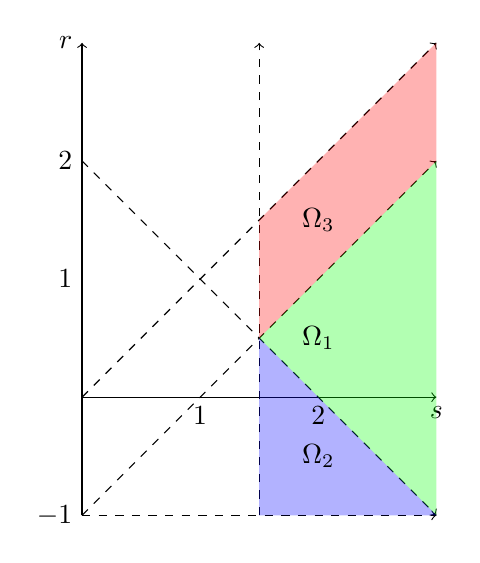
\begin{tikzpicture}[scale=1.5]
% Draw thin grid lines with color 40% gray + 60% white
% Draw x and y axis lines
\draw [->] (0,0) -- (3,0) node [below] {$s$};
\draw [->] (0,-1) -- (0,3) node [left] {$r$};
\draw [->, dashed] (0,0) -- (3,3);
\draw [->, dashed] (0,-1) -- (3,2);
\draw [->, dashed] (0,2) -- (3,-1);
\draw [->, dashed] (0,-1) -- (3,-1);
\draw [->, dashed] (3/2,-1) -- (3/2, 3);
\fill[color=green, fill opacity=0.3] (1.5, 0.5) -- (3,2) -- (3,0) -- (3,-1);
\fill[color=red, fill opacity=0.3] (1.5, 0.5) -- (1.5,1.5) -- (3,3) -- (3,2);
\fill[color=blue, fill opacity=0.3] (1.5, 0.5) -- (1.5, -1) -- (3, -1);
\foreach \x/\xtext in {1, 2}
\draw[shift={(\x,0)}]  node[below] {$\xtext$};
\foreach \y/\ytext in {-1, 1, 2}
\draw[shift={(0,\y)}]  node[left] {$\ytext$};
\draw (2,1.5) node {$\Omega_{3}$};
\draw (2,0.5) node {$\Omega_{1}$};
\draw (2,-0.5) node {$\Omega_{2}$};
\end{tikzpicture}
\end{center}
%
\end{frame}
\begin{frame}
%
Then for two initial data $u_{0}, v_{0} \in B_{H^{s}}(R)$, there exist unique
corresponding solutions \\ $u(x,t), v(x,t)$ for $0 \le t \le T= T(R)$ to the
HR equation which satisfy 
%
%
\begin{equation*}
\begin{split}
\| u(t) - v(t) \|_{H^{r}} \le C \| u_{0} - v_{0} \|_{H^{r}}^{\alpha(s, r)},
\quad 0
\le t \le T
\end{split}
\end{equation*}
%
%
where 
%
%
\begin{equation*}
\begin{split}
\alpha = 
\begin{cases}
1, \quad & (s,r) \in \Omega_{1} 
\\
2(s-1)/(s-r),  \quad & (s, r) \in \Omega_{2}
\\
s-r, \quad & (s, r) \in \Omega_{3}.
\end{cases}
\end{split}
\end{equation*}
%
%
%%%%%%%%%%%%%%%%%%%%%%%%%%%%%%%%%%%%%%%%%%%%%%%%%%%%%
%
%
%                Main theorem
%
%
%%%%%%%%%%%%%%%%%%%%%%%%%%%%%%%%%%%%%%%%%%%%%%%%%%%%%
%
%
\pause
$\bullet$ This result sharper than analogue obtained in
work of Chen for $b$-family. 
\\
$\bullet$ Techniques applied here can be applied to sharpen results in their paper. 
\end{frame}
\begin{frame}
  \frametitle{Method of Proof}
 $\bullet$ Use energy estimates. 
 \\
 $\bullet$
 Need commutator estimate and multiplier estimate. Able to obtain
\begin{equation*}
\begin{split}
\frac{1}{2} \frac{d}{dt}
\|v\|_{H^r}^2
& \lesssim \|u+w\|_{H^s}
\|v\|_{H^r}^2, \quad | t | < T.
\label{9v-iu}
\end{split}
\end{equation*}
in $\Omega_{1}$, for example. Gives Lip dependence.
\\
\pause
$\bullet$
H\"older dependence in remaining regions follow from the above and Sobolev interpolation.
\end{frame}
\begin{thebibliography}{HKM09}

\bibitem[Die69]{Dieudonne_1969_Foundations-of-}
J.~Dieudonn{{\'e}}, \emph{Foundations of modern analysis}, Academic Press, New
  York, 1969, Enlarged and corrected printing, Pure and Applied Mathematics,
  Vol. 10-I. 

\bibitem[Fol99]{Folland_1999_Real-analysis}
G.~B. Folland, \emph{Real analysis}, second ed., Pure and Applied
  Mathematics (New York), John Wiley \& Sons Inc., New York, 1999, Modern
  techniques and their applications, A Wiley-Interscience Publication.
  

\bibitem[HK09]{Himonas_2009_Non-uniform-dep}
A. Himonas and C.~E. Kenig, \emph{Non-uniform dependence on initial data
  for the ch equation on the line}, Differential Integral Equations \textbf{22}
  (2009), no.~3-4, 201--224.

\bibitem[HKM10]{Himonas:2010}
A. Himonas, C.~Kenig, and G.~Misio{\l}ek, \emph{Non-uniform dependence for the
  periodic {CH} equation}, Comm. Partial Differential Equations \textbf{35}
  (2010), no.~6, 1145--1162. 

\bibitem[KP88]{Kato_1988_Commutator-esti}
T. Kato and G. Ponce, \emph{Commutator estimates and the {E}uler and
  {N}avier-{S}tokes equations}, Comm. Pure Appl. Math. \textbf{41} (1988),
  no.~7, 891--907. 

\bibitem[Tay91]{Taylor_1991_Pseudodifferent}
M.~E. Taylor, \emph{Pseudodifferential operators and nonlinear {PDE}},
  Progress in Mathematics, vol. 100, Birkh{\"a}user Boston Inc., Boston, MA,
  1991. 

\bibitem[Tay03]{Taylor_2003_Commutator-esti}
M.~E. Taylor, \emph{Commutator estimates}, Proc. Amer. Math. Soc.
  \textbf{131} (2003), no.~5, 1501--1507 (electronic). 
 
\bibitem[CLZ11]{Chen:2011fk}
R.~M. Chen, Y.~Liu, and P.~Zhang, \emph{The h{\"o}lder continuity of the
  solution map to the {\$}b{\$}-family equation in weak topology}, submitted,
  2011.

\end{thebibliography}

\begin{frame}
  \begin{center}\Large THANK YOU!
  \\
  (Stay Cool)

    \includegraphics[scale=0.6]{./cat-sunglasses.jpg}
\end{center}
\end{frame}
%\bibliographystyle{amsalpha}
%\bibliography{/Users/davidkarapetyan/Documents/math/references.bib}
%\nocite{*}

 \end{document}


